\documentclass[12pt,a4paper]{article}

\usepackage[utf8]{vietnam}
%\usepackage[utf8]{inputenc}
%\usepackage[vietnam]{babel}    %tạo bảng trong tài liệu
\usepackage{amsmath}
%\usepackage{hyperref}     %tạo khung tròn từng đầu mục trong mục lục
\usepackage{listings}
\usepackage{amsfonts}
\usepackage{dsfont}
\usepackage{amssymb}
\usepackage{graphicx}
\usepackage{setspace} %khoảng cách giữa các dòng
\usepackage{xcolor}      %thêm màu cho text	
%\usepackage{draftwatermark}     %chèn watermark
%\SetWatermarkText{Giải tích số}
%\SetWatermarkScale{0.6}  %% kích cỡ chữ muốn chèn
\usepackage[left=2cm,right=2cm,top=2cm,bottom=2cm]{geometry}

\usepackage{fancyhdr}      %thêm header và footer
\pagestyle{fancy}      %kiểu trang khi thêm header và footer, có 2 thanh đen, 1 thanh dưới header, 1 thanh trên footer (*)
\usepackage{utopia}    %in đậm các câu đầu thư mục, câu lệnh chính.
\usepackage{listings}  %chen code
\lhead{\textbf{Giải tích số}}     %lệnh textbf: dùng để in đậm chữ
\chead{}
\rhead{\textbf{\textit{Viện Toán Ứng Dụng và Tin Học}}}    %lệnh textit: dùng để in nghiêng chữ
\lfoot{\textbf{Báo cáo nhóm 5 - Toán tin 2-K59}}
\cfoot{}
\rfoot{\textbf{\thepage}}
\renewcommand{\headrulewidth}{0.4pt}
\renewcommand{\footrulewidth}{0.4pt} 

\definecolor{dkgreen}{rgb}{0,0.6,0}
\definecolor{gray}{rgb}{0.5,0.5,0.5}
\definecolor{mauve}{rgb}{0.58,0,0.82}

\lstset{frame=tb,
  language=C++,
  aboveskip=3mm,
  belowskip=3mm,
  showstringspaces=false,
  columns=flexible,
  basicstyle={\small\ttfamily},
  numbers=none,
  numberstyle=\tiny\color{gray},
  keywordstyle=\color{blue},
  commentstyle=\color{dkgreen},
  stringstyle=\color{mauve},
  breaklines=true,
  breakatwhitespace=true,
  tabsize=3
}  % chen code

\begin{document} %thiết lập lệnh bắt đầu cho tài liệu
\fontsize{12}{16}\selectfont %định cỡ chữ và khoảng cách các dòng sau \selectfont
\pagenumbering{gobble}   %ko đánh số trang ở lời mở đầu

\author{Giảng viên hướng dẫn: Lê Thị Ngọc Yến}    %tên tác giả
\title{Đề tài báo cáo}    %tiêu đề tài liệu

\title{BÁO CÁO MÔN HỌC \\Sử dụng phương pháp lặp Seidel và Gauss-Seidel (cho hệ chéo trội) để giải hệ phương trình đại số tuyến tính}
\date{\today{}}  %thiết lập ngày giờ là ngày hôm nay

\maketitle{}   %tạo tiêu đề
\begin{center}       %chèn hình: logo bách khoa
    \begin{figure}[htp]
    \begin{center}
     
\includegraphics[scale=.2]{logo}
    \end{center}
    %\caption{}
    \label{}
    \end{figure}
\end{center}

\\
\begin{center}
%\setstretch{4.0}
%\doublespacing
%\setlength{\parindent}{giá_trị_khoảng_cách}
Nhóm báo cáo: \\ 

1. Phan Huy Hoàng ( nhóm trưởng ) - Toán Tin 2-K59\\

2. Trần Thị Thanh Tâm - Toán Tin 2-K59\\

3. Nguyễn Văn Thành Dũng - Toán Tin 2-K59\\

\end{center} 

\newpage   %sang trang mới

\pagenumbering{arabic}     %đánh số trang là số
%muốn đánh số trang bằng số la mã, thay bằng "roman"

\tableofcontents{}    %tạo mục lục

\newpage
%////////////////////////////////////////////////////////////////////////////////////
%\title{\textbf{CHƯƠNG 1}}\\
%\title{\textbf{KHÔNG GIAN METRIC}}

\section{Lời mở đầu }
\hspace{0.7cm}- Sau khi học các môn học cơ sở ngành như: Tin học đại cương, Kĩ Thuật Lập Trình và Cơ sở Giải Tích Hàm, dưới sự hướng dẫn của giáo viên bộ môn Giải Tích Số, cô Hà Thị Ngọc Yến, chúng em đã tiến hành tìm hiểu nội dung đề tài để viết nên báo cáo này. Đề tài của nhóm em là: {\color{red}Tìm hiểu phương pháp lặp Seidel và Gauss-Seidel để giải hệ phương trình đại số tuyến tính}. \\

- Nội dung chính của báo cáo bao gồm những phần cơ bản như: lý thuyết cơ bản, các định nghĩa và định lý trong đề tài, code chương trình và chạy chương trình trên máy,..... \\

- Như chúng ta đã biết, để giải hệ phương trình đại số tuyến tính ( ĐSTT ), chúng ta có 2 phương pháp chính cơ bản như sau: phương pháp giải đúng ( như Gauss, Gauss-Jordan,...) và phương pháp giải gần đúng ( như lặp đơn, Seidel, Gauss-Seidel). Trong báo cáo này ta sẽ đề cập tới phương pháp giải gần đúng Seidel và Gauss-Seidel cho hệ phương trình ĐSTT, những ưu điểm, hạn chế của phương pháp so với phương pháp lặp đơn, khi nào và tại sao sử dụng phương pháp này,...\\

- Vì cũng là lần đầu tìm hiểu đề tài, thời gian tìm hiểu tương đối ngắn, hơn nữa cũng là 1 trong 2 nhóm thuyết trình đầu tiên nên báo cáo do nhóm thực hiện không tránh khỏi những thiếu sót ( cả về mặt trình bày và nội dung báo cáo ). Với khả năng có hạn nên có thể trong báo cáo chưa trình bày được đầy đủ nội dung chương trình, cũng mong giáo viên bộ môn góp ý và lượng thứ.\\

\begin{center}
\\ \textbf{--- Tài liệu được viết bằng LATEX, 24/02/2016 ---}\\
\end{center} 



\newpage



\section{Bài toán đặt ra}\\
\hspace{0.7cm}\textbf{Chuẩn vectơ và sự hội tụ của dãy vectơ}\\ 

- Mục đích của phương pháp tìm nghiệm gần đúng của hệ đại số tuyến tính là: xuất phát từ vectơ $X^{(0)}$ gọi là xấp xỉ đầu, tìm cách hiệu chỉnh dần sau một số bước ta thu được dãy vectơ $\{X^{(k)}\}$ mà vectơ $X^{(0)}$ gần đúng với nghiệm đúng của hệ. Vì vậy cần thiết phải đưa vào khái niệm về sự hội tụ của dãy vectơ.Khái niệm đơn giản và dễ hình dung nhất là {\color{red}sự hội tụ theo tọa độ}.
\begin{itemize}
\item {\textbf{Định nghĩa 1}: Dãy vectơ $X^{(k)} = (x_1^{(k)}, x_2^{(k)}, ..., x_n^{(k)})^t$ với $k = 1, 2,...$ trong không gian n chiều, hội tụ tới vectơ $X = (x_1, ... ,x_n)^t \in R^n$ nếu: \\}
$$\left| x_i^{(k)} - x_i \right| \rightarrow 0 \enskip khi \enskip k \rightarrow \infty \enskip \forall i = \overline{1,n}$$

- Và kí hiệu ${\lim }\limits_{x \to \infty } \ X^{(k)} = X$.
%\[\mathop {\lim }\limits_{x \to \infty } \X^{(k)} = X \] : căn ra giữa dòng

- Sự hội tụ như vậy gọi là {\color{red}hội tụ theo tọa độ}.

- Tuy vậy khái niệm này khó sử dụng, ta sẽ sử dụng sự hội tụ theo nghĩa khác mà hệ quả của nó cũng là sự hội tụ theo tọa độ. Để mô tả sự hội tụ này trước hết ta gán cho mỗi vectơ $X$ n chiều một số thực không âm $N(x)$ mà ta gọi là chuẩn của vectơ $X$. 

\item{\textbf{Định nghĩa 2}: Ta gọi {\color{red}chuẩn của vectơ $X$}, ký hiệu $||X|| = N(X) $ là một số không âm thỏa mãn điều kiện sau: }
%\[ B(a, r ) = \lbrace x \in X: d(a,x ) < r  & ( r >0 )  \\ \] 
%đánh số 1,2,3
\begin{enumerate}
\item {$||X|| = N(X) \geq 0$, $"= 0" \Leftrightarrow X = 0$}
\item {$||kX|| = N(kX) = |k|||X||$, $\quad k - const$}
\item {$||X + Y|| = N(X + Y) \leq ||X|| + ||Y||$}
\end{enumerate}

( X, Y là những vectơ n chiều )

- Như vậy, $||X|| = N(X)$ có thể xem như độ dài của vectơ $X$ và các điều kiện 1, 2, 3 của nó giống tính chất độ dài hình học của vectơ hình học.

- Thông thường, ta có 3 loại chuẩn như sau:

{\color{red}( Chuẩn cực đại )} $$ ||X||_{(\infty)} = max_i {|x_i|} $$ 

{\color{red}( Chuẩn tuyệt đối )} $$ ||X||_{(1)} = \sum\limits_{i = 1}^n {|x_i|} $$

{\color{red}( Chuẩn Ơcơlit )} $$ ||X||_{(2)} = {\left[ \begin{matrix} \sum\limits_{i = 1}^n {|x_i^2|} \end{matrix}\right]}^{\frac{1}{2}} $$

- Dễ dàng chỉ ra rằng các chuẩn trên thỏa mãn các điều kiện 1, 2, 3.

\item{\textbf{Định nghĩa 3}: Ta nói dãy vectơ $\{X^{(k)}\} = \{(x_1^{(k)}, x_2^{(k)}, ..., x_n^{(k)})^t\}$ hội tụ tới vecto $X = (x_1, x_2, ..., x_n)^t$, nếu theo chuẩn nào đó ta có $||X^{(k)} - X|| \rightarrow 0$ khi $k \rightarrow \infty$.\\

- Với 3 loại chuẩn đã xét thì dễ dàng chứng minh được định nghĩa 1 và định nghĩa 3 tương đương.

- Bây giờ xét ma trận $A = [a_{ij}]$ là ma trận vuông cấp n, ta cũng có:

\item{\textbf{Định nghĩa 4}: Ta gọi {\color{red}chuẩn của ma trận $A$}, ký hiệu $||A||$ (đọc là chuẩn của ma trận $||A||$) là số không âm thỏa mãn các điều kiện sau:}

\begin{enumerate}
\item {$||A|| \geqslant 0 \quad "= 0" \Leftrightarrow A = 0 $ (ma trận không)}
\item {$||kA|| = |k|||A||$, $k = const$}
\item {$||A + B|| \leqslant ||A|| + ||B||$}
\end{enumerate}

(A, B là những ma trận vuông cấp n)

- Các chuẩn của ma trận $A$ thường được chọn:

{\color{red}(theo hàng)} $$ ||A||_{(\infty)} = max_i \sum\limits_{j = 1}^n {a_{ij}} $$ 

{\color{red}(theo cột)} $$ ||A||_{(1)} = max_i \sum\limits_{i = 1}^n {a_{ij}} $$  

{\color{red}(chuẩn Ơcơlit)}  $$ ||A||_{(2)} = {\left[ \begin{matrix} \sum\limits_{i = 1}^n {\sum\limits_{j = 1}^n {a_{ij}^2 } \end{matrix}\right]}^{\frac{1}{2}} $$

- Dễ dàng chỉ ra rằng 3 dạng chuẩn trên thỏa mãn các điều kiện về chuẩn; đồng thời ta cũng có:

\[ ||AB|| \leqslant ||A||||B|| \Rightarrow ||A^m|| \leqslant ||A||^m\]

\item{\textbf{Định nghĩa 5}: Dãy ma trận $\{A^{(k)}\} = \{(a_{ij}^{(k)})_{i,j = \overline{1n}}\}$\\

- $k = 1, 2,...$ hội tụ tới ma trận $A = (a_{ij})_n$ khi $ k \rightarrow\infty$ nếu $\mathop {\lim }\limits_{k \to \infty } \a_{ij}^{(k)} = a_{ij}$, $\forall ij$ (hội tụ theo dãy các phần tử

hoặc $||A^{(k)} - A|| \rightarrow 0$ khi $ k\rightarrow\infty $ (hội tụ theo chuẩn)

- Kí hiệu $\mathop {\lim }\limits_{k \to \infty } A^{(k)}} = A$

- Trong bài toán phần lớn thường có sự tham gia của cả ma trận và vectơ: \\ 

$$ AX = {\left[ \begin{matrix} \sum\limits_{j = 1}^n {{a_{ij}.x_j}} \end{matrix}\right]}_{i = \overline{1,n}}$$ ( là vectơ cột )

\end{itemize}

\newpage

\section{Phương pháp lặp Seidel}

\hspace{0.7cm- }Phương pháp lặp Seidel đặt ra nhằm mục đích {\color{red}tiết kiệm ô nhớ trong máy tính}, đồng thời cũng là {\color{red}tranh thủ tối đa lượng thông tin đã có trong quá trình tính}.\\

- Xét hệ phương trình đại số tuyến tính (ĐSTT):
%đánh số phép tính 
\begin{align}
X = \alpha X + \beta
\end{align}

- Ta phân tích ma trận $\alpha$ thành: $\alpha = {\alpha}^{(1)} + {\alpha}^{(2)}$:

$$ \alpha = \left( {\begin{array}{*{20}{c}}
{{a_{11}}}& \ldots &{{a_{1n}}}\\
 \vdots & \ddots & \vdots \\
{{a_{n1}}}& \cdots &{{a_{nn}}}
\end{array}} \right) = \left( {\begin{array}{*{20}{c}}
0&{... \ldots }&0\\
 \vdots &0& \vdots \\
{{a_{n1}}}& \cdots &0
\end{array}} \right) + \left( {\begin{array}{*{20}{c}}
{{a_{11}}}& \ldots &{{a_{1n}}}\\
 \vdots & \ddots & \vdots \\
0& \cdots &{{a_{nn}}}
\end{array}} \right)$$

- Từ $(1)$ ta có:
$$  X = \alpha X + \beta = [{\alpha}^{(1)} + {\alpha}^{(2)}]X + \beta  $$
\begin{align}
hay: X = {\alpha}^{(1)}X + {\alpha}^{(2)}X + \beta
\end{align}

\begin{itemize}
\item {\textbf{Thuật toán}: Chọn xấp xỉ đầu là $X^{(0)}$ bất kỳ, tính:  \\}
%\left \{
$$\left\{\begin{matrix} {x_1^{(1)} = \sum\limits_{j = 1}^n {{{\alpha}_{1j}.x_j^{(0)}}}  + {\beta}_1}\\{x_2^{(1)} = {\alpha}_{21}.x_1^{(1)} + \sum\limits_{j = 2}^n {{{\alpha}_{2j}.x_j^{(0)}}}  + {\beta}_2}\\{..........}\\{x_n^{(1)} = \sum\limits_{j = 1}^{i - 1} {{{\alpha}_{ij}.x_j^{(1)}}} + \sum\limits_{j = i}^{n} {{{\alpha}_{ij}.x_j^{(0)}}} + {\beta}_j}\\{..........}\\{x_n^{(1)} = \sum\limits_{j = 1}^{n - 1} {{{\alpha}_{nj}.x_j^{(1)}}} + {\alpha}_{nn}.x_n^{(0)} + {\beta}_n} \end{matrix} $$

hay: $$ x_i^{(1)} = \sum\limits_{j = 1}^{i - 1} {{{\alpha}_{ij}.x_j^{(1)}}} + \sum\limits_{j = i}^{n} {{{\alpha}_{ij}.x_j^{(0)}}} + {\beta}_j \qquad i = 1,2,...,n \\$$

- Sau bước một, ta được xấp xỉ thứ nhất $X^{(1)}$:
$$X^{(1)} = (x_1^{(1)}, x_2^{(1)}, ..., x_n^{(1)})^t $$

-Lặp lại quá trình trên đối với $X^{(1)}$, ta được $X^{(2)}$, ....cứ như vậy đến phép lặp thứ $k$, ta có:
\begin{align}
x_i^{(k)} = \sum\limits_{j = 1}^{i - 1} {{{\alpha}_{ij}.x_j^{(k)}}} + \sum\limits_{j = i}^{n} {{{\alpha}_{ij}.x_j^{(k - 1)}}} + {\beta}_j \qquad i = \overline{1,n} \qquad k = 1,2,.....
\end{align}


hay:\begin{align}
X^{(k + 1)} = {\alpha}^{(1)}X^{(k + 1)} + {\alpha}^{(2)}X^{(k)} + \beta \qquad k = 0,1,2,.....
\end{align}

\newpage

\item {\textbf{Điều kiện hội tụ và sai số}: Nếu quá trình lặp $(4)$ hội tụ thì: $\mathop {\lim }\limits_{x \to \infty } x^{(k)} = \overline{X}$ thì $\overline{X} = X^{*}$ là nghiệm đúng của hệ $(1)$ hay $(2)$\\}

- Thực vậy, từ $(4)$, do $X^{(k)} \rightarrow \overline{X}$ khi $X \rightarrow \infty $ nên:
$$ \overline{X} = {\alpha}^{(1)}\overline{X} + {\alpha}^{(2)}\overline{X} + \beta = (\alpha}^{(1)} + \alpha}^{(2)})\overline{X} + \beta $$
hay: $$ \overline{X} = \alpha\overline{X} + \beta $$
vậy: $$ \overline{X} = X^{*}$$ 

- Điều kiện để quá trình lặp $(4)$ hội tụ và sai số.

\textbf{Định lí 1}: Nếu một chuẩn nào đó của ma trận $\alpha$ thỏa mãn điều kiện: 
$$||\alpha||_{(p)} < 1 \qquad (p = \infty, 1)$$
thì phương pháp lặp Seidel hội tụ tới nghiệm đúng $X^{*}$ của hệ phương trình $(1)$ với nghiệm xấp xỉ đầu $X^{(0)}$ bất kỳ.

- Đồng thời ta có các công thức đánh giá sai số:

\textbf{a) Nếu ${\color{red}||\alpha||_{\infty} < 1}$ thì:}
\begin{align}
||X^{(k)} - X^*||_{\infty} < \frac{\lambda}{1 - \lambda} ||X^{(k)} - X^{(k - 1)}||_{\infty}
\end{align}
trong đó:$$ \lambda = max_i \frac{{\sum\limits_{j = i}^n {{|{\alpha}_{ij}|}} }}{1 - \sum\limits_{j = i}^{i - 1} {|{\alpha}_{ij}|}}} \leqslant ||\alpha||_{\infty} < 1$$

hoặc: 
\begin{align}
||X^{(k)} - X^{*}||_{\infty} < \frac{||\alpha||^k}{1 - ||\alpha||} ||X^{(1)} - X^{0}||_{\infty}
\end{align}

\textbf{b) Nếu ${\color{red}||\alpha||_{(1)} < 1}$ thì:}
\begin{align}
||X^{(k)} - X^{*}||_{1} < \frac{{\zeta}^k}{(1 - S)(1 - \zeta)} ||X^{(1)} - X^{0}||_{(1)}
\end{align}
trong đó:$$S = max_i \sum\limits_{i = j + 1}^n {{|{\alpha}_{ij}|}}; \qquad \zeta = \quad max_j \frac{{\sum\limits_{i = 1}^j {{|{\alpha}_{ij}|}} }}{1 - \sum \limits_{i = j + 1}^{n} {|{\alpha}_{ij}|}}} \leqslant ||\alpha||_{(1)} < 1 $$

\textbf{CHỨNG MINH: }Khi $||\alpha||_{(\infty)} < 1$ - theo $(3)$, ta có: $$ x_i^{(k)} = \sum\limits_{j = 1}^{i - 1} {{{\alpha}_{ij}.x_j^{(k)}}} + \sum\limits_{j = i}^{n} {{{\alpha}_{ij}.x_j^{(k - 1)}}} + {\beta}_j \qquad i = \overline{1n}; k = 1,2,.....\\$$

- Nếu $X^{*}$ là nghiệm đúng của phương trình $(1)$ thì:
$$ x_1^{*} = \sum\limits_{j = 1}^n {{{\alpha}_{ij}.x_j^{*}}}  + {\beta}_j \qquad i = \overline{1n} $$

$$\Longrightarrow x_i^{(k)} - x_i^{*} = \sum\limits_{j = 1}^{i - 1} {{|{\alpha}_{ij}|}(x_j^{(k)} - x_j^{*})} + \sum\limits_{j = i}^n {{|{\alpha}_{ij}|}(x_j^{(k - 1)} - x_j^{*})} $$

\begin{align}
\Longrightarrow|x_i^{(k)} - x_i^{*}| \leqslant {\sum\limits_{j = 1}^{i - 1}{{{\alpha}_{ij}} |(x_j^{(k)} - x_j^{*})| + \sum\limits_{j = i}^n {{{\alpha}_{ij}} |(x_j^{(k - 1)} - x_j^{*})| \qquad i = \overline{1n}}}}
\end{align} 

- Đặt $P_i = \sum\limits_{j = 1}^{i - 1} {{|{\alpha}_{ij}|}}; \qquad q_i = \sum\limits_{j = i}^n {{|{\alpha}_{ij}|}}; $

mà $\forall j: \qquad |x_i^{(k)} - x_i^{*}| \leqslant ||X^{(k)} - X^{*}||_{\infty}$ nên từ $(9)$:
\begin{align}
|x_i^{(k)} - x_i^{*}| \leqslant P_i ||X^{(k)} - X^{*}||_{\infty} + q_i ||X^{(k - 1)} - X^{*}||_{\infty}
\end{align}
giả sử với vectơ $X^{(k)}$, có chỉ số s nào đó mà: 
$$ |x_s^{(k)} - x_s^{*}| = max_i |x_i^{(k)} - x_i^{*}| =||X^{(k)} - X^{*}||_{\infty} $$ thì từ $(9)$ ta có:
$$ ||X^{(k)} - X^{*}||_{\infty} \leqslant p_s ||X^{(k)} - X^{*}||_{\infty} + q_s ||X^{(k - 1)} - X^{*}||_{\infty}$$
hay $$ ||X^{(k)} - X^{*}||_{\infty} \leqslant \frac{q_s}{1 - p_s} ||X^{(k - 1)} - X^{*}||_{\infty}$$

- Đặt \begin{align}
\lambda = max_i\frac{q_i}{1 - p_i} = max_i \frac{\sum\limits_{j = i}^n {{|{\alpha}|_{ij}}}}{1 - \sum\limits_{j = 1}^{i - 1} {{|{\alpha}|_{ij}}}}
\end{align} 
\begin{align}
\Longrightarrow ||X^{(k)} - X^{*}||_{\infty} \leqslant \lambda ||X^{(k - 1)} - X^{*}||_{\infty} 
\end{align}

- Ta sẽ chứng minh: $\lambda \leqslant ||\alpha||_{\infty} < 1$

- Ta có: $p_i + q_i = \sum\limits_{j = 1}^n {{|{\alpha}_{ij}|}} \leqslant ||\alpha||_{\infty} < 1$ theo giả thiết ta đặt ra ban đầu nên $q_i \leqslant ||\alpha||_{\infty} - p_i \Rightarrow \forall i = \overline{1n}$ ta có:
$$ \frac{q_i}{1 - p_i} < \frac{||\alpha||_{\infty} - p_i}{1 - p_i} \leqslant \frac{||\alpha||_{\infty} - p_i ||\alpha||_{\infty}}{1 - p_i} = ||\alpha||_{\infty} < 1$$

hay $$ \lambda = max_i \frac{q_i}{1 - p_i} \leqslant ||\alpha||_{\infty} < 1$$

- Với biểu thức $(12)$, lặp k lần ta được: 
$$ ||X^{(k)} - X^{*}||_{\infty} \leqslant \lambda ||X^{(k - 1)} - X^{*}||_{\infty} \leqslant ..... \leqslant {\lambda}^k ||X^{(0)} - X^{*}||_{\infty}$$
$$ \longrightarrow ||X^{(k)} - X^{*}||_{\infty} \rightarrow 0 \qquad khi \qquad k \rightarrow \infty $$ 
hay $ \mathop {\lim }\limits_{x \to \infty } \ X^{(k)} = X^* $ là điều phải chứng minh.

- Quay trở lại, ta sẽ chứng minh 2 công thức sai số $(5)$ và $(6)$ 

- Xét phép lặp liên tiếp của $X^{(k + 1)}$ và $X^{(k)}$, tương tự như trên, ta có:
\begin{align}
||X^{(k + 1)} - X^{k}||_{\infty} \leqslant \lambda ||X^{(k)} - X^{k - 1}||_{\infty}
\end{align}

- Với p nguyên dương bất kì, ta có:
$$||X^{(k + p)} - X^{k}||_{\infty} \leqslant ||X^{(k + p)} - X^{(k + p - 1)}||_{\infty} + ... + ||X^{(k + 1)} - X^{(k)}||_{\infty} $$
\begin{align}
\leqslant ({\lambda}^p + {\lambda}^{p - 1} + ... + \lambda)||X^{(k)} - X^{(k - 1)}||_{\infty}  
\end{align}
$$ \leqslant \lambda \frac{1 - {\lambda}^p}{1- \lambda} ||X^{(k)} - X^{(k - 1)}||_{\infty}$$

- Cố định k, cho $p \rightarrow \infty$ thì $X^{k + p} \rightarrow X^*$. Từ $(13)$ có:
$$ ||X^{*} - X^{(k)}||_{\infty} \leqslant \frac{\lambda}{1 - \lambda} ||X^{(k)} - X^{(k - 1)}||_{\infty}$$

$\Longrightarrow$ BĐT $(5)$ được chứng minh.\\

\textbf{- Với BĐT $(6)$, ta lấy BĐT $(12)$ với $k$ là $k + p - 1$ }
$$ ||X^{(k + p)} - X^{(k + p - 1)}||_{\infty} \leqslant \lambda ||X^{(k + p - 1)} - X^{(k + p - 2)}||_{\infty}$$

- Lặp p lần, ta được:
\begin{align}
||X^{(k + p)} - X^{(k + p - 1)}||_{\infty} \leqslant {\lambda}^p ||X^{(k)} - X^{(k - 1)}||_{\infty}
\end{align}

- Trong BĐT $(14)$ chọn k = 1:
$$ ||X^{(1 + p)} - X^{(p)}||_{\infty} \leqslant {\lambda}^p ||X^{(1)} - X^{(0)}||_{\infty} $$

tiếp tục thay $p = k - 1$ ta được: 
$$ ||X^{(k)} - X^{(k - 1)}||_{\infty} \leqslant {\lambda}^{k - 1} ||X^{(1)} - X^{(0)}||_{\infty} $$

thay vào BĐT $(5)$, ta có:
$$ ||X^{(k)} - X^{(*)}||_{\infty} \leqslant \frac{\lambda}{1 - \lambda} ||X^{(k)} - X^{(k - 1)}||_{\infty} \leqslant \frac{{\lambda}^k}{1 - \lambda} ||X^{(1)} - X^{(0)}||_{\infty} $$

$\Longrightarrow$ BĐT $(6)$ được chứng minh.\\

\item{\textbf{NHẬN XÉT CHUNG: }}

- Phương pháp Seidel có {\color{red}độ chính xác cao} và {\color{red}tốc độ hội tụ nhanh hơn} phương pháp lặp đơn (vì $\lambda < ||\alpha|| < 1$ )

- Phương pháp Seidel {\color{red}tiết kiệm bộ nhớ hơn} phương pháp lặp đơn vì: 
\begin{itemize}
\item[$\nabla$]{Phương pháp lặp đơn sử dụng 2n ô nhớ cho $X^{(k + 1)}$ và $X^{(k)}$.
\item[$\nabla$]{Trong khi đó, phương pháp Seidel {\color{red}chỉ cần $n$ ô nhớ cho $X^{(k)} \rightarrow X^{(k + 1)}$}. Vì giả sử sau khi tính $X_1^{(k + 1)}$ thì không cần sử dụng $X^{(k)}$, lúc đó bỏ số $X_1^{(k + 1)}$ vào ô nhớ của $X^{(k)}$ để tính $X_1^{(k + 2)}$,....cứ như vậy...\\}
\end{itemize}

\item{\textbf{VÍ DỤ: }}: Tìm nghiệm gần đúng của phương trình sau bằng phương pháp lặp Seidel: 
$$ \left\{\begin{matrix} 1.02x_1 - 0.05x_2 - 0.1x_3 = 0.795\\-0.11x_1 + 1.03x_2 - 0.05x_3 = 0.849\\ -0.11x_1 + 0.12x_2 - 0.04x_3 = 1.398 \end{matrix} $$

\textbf{Giải }: 

- Hệ $\Leftrightarrow$ $ \left\{\begin{matrix} x_1 = -0.02x_1 + 0.05x_2 + 0.1x_3 + 0.795\\x_2 = 0.11x_1 - 0.03x_2 + 0.05x_3 + 0.849\\ x_3 = 0.11x_1 + 0.12x_2 - 0.04x_3 + 1.398 \end{matrix} \Rightarrow \left( {\begin{array}{*{20}{c}}
{ - 0.02}&{0.05}&{0.1}\\
{0.11}&{ - 0.03}&{0.05}\\
{0.11}&{0.12}&{ - 0.04}
\end{array}} \right) \\ $ \\ 

\\

- Với $ B_1 = \left( {\begin{array}{*{20}{c}}
{ 0}&{0}&{0}\\
{0.11}&{0}&{0}\\
{0.11}&{0.12}&{ 0}
\end{array}} \right)$ ; 
$\qquad B_2 = \left( {\begin{array}{*{20}{c}}
{ - 0.02}&{0.05}&{0.1}\\
{0}&{ - 0.03}&{0.05}\\
{0}&{0}&{ - 0.04}
\end{array}} \right) \\ $ \\

\\

- Xét phép lặp $X_{(k + 1)} = B_1 X_{(k + 1)} + B_2 X_{(k)} + g$ \\

$\Leftrightarrow \left\{\begin{matrix} x_1^{(k + 1)} = ( -0.02x_1^k + 0.05x_2^k + 0.1x_3^k ) + 0.795\\x_2^{(k + 1)} = 0.11x_1^{k + 1} + ( -0.03x_2^k + 0.05x_3^k ) + 0.849\\ x_3^{(k + 1)} = 0.11x_1^{(k + 1)} + 0.12x_2^{(k + 1)} - 0.04x_3^{(k + 1)} + 1.398 \end{matrix} \\ $ \\

\\ $ \begin{matrix} k&|&x_1^k&x_2^k&x_3^k\\ 0&|&0.8&0.85&1.4 \\ 1&|&0.9615&0.999265&1.56767\\ 2&|&0.9825&1.00548&1.564025 \\.................... \end{matrix} \\ $

\end{itemize}

\newpage



\section{Phương pháp lặp Gauss - Seidel}

\begin{itemize}
\item{ \textbf{Đinh nghĩa }}: Là phương pháp Seidel áp dụng cho hệ phương trình đại số tuyến tính với {\color{red}ma trận đường chéo trội}.

$ \Rightarrow$ Vậy thế nào là ma trận đường chéo trội ???

\item{ \textbf{Ma trận đường chéo trội}}: {\color{red}Ma trận đường chéo trội} là ma trận thỏa mãn:

$$ |a_{ij}| > \sum\limits_{i = 1, j \neq i}^n {{|a_{ij}|}} \qquad i = \overline{1,n}$$

- Trường hợp cụ thể, phương trình $AX = B$, trong đó ma trận hệ số $A$ có đường chéo trội thì quá trình lặp Seidel được tính như sau: chọn xấp xỉ đầu $X^{(0)} = (x_1^{(0)}, x_1^{(1)}, ...., x_1^{(n)})^t$ thì: 

\begin{align}
x_i^{(k + 1)} = \frac{1}{a_{ii}} {\left[ \begin{matrix} \sum\limits_{j = 1}^{i - 1} {{a_{ij}x_j^{(k + 1)}}} + \sum\limits_{j = i + 1}^n {{a_{ij}x_j^{(k)}}}  \end{matrix}\right]} + \frac{a_{i, {n + 1}}}{ii} \qquad i = \overline{1n} \qquad k = 0,1,2,.....
\end{align}

\item{\textbf{VÍ DỤ: }}: Tìm nghiệm gần đúng của phương trình sau bằng phương pháp lặp Seidel - Gauss Seidel: 

$$ \left\{\begin{matrix} 4x_1 - 2.4x_2 - 0.8x_3 = 8\\0.9x_1 + 3x_2 - 1.5x_3 = 9\\ 0.4x_1 - 0.8x_2 + 4x_3 = 20 \end{matrix} $$

\textbf{Giải: }: Dễ thấy hệ phương trình đã cho có dạng đường chéo trội 

$$ |a_{ij}| > \sum\limits_{i = 1, j \neq i}^n {{|a_{ij}|}} \qquad i = \overline{1,n}$$

nên dễ dàng đưa được về dạng $X = \alpha X + \beta$, trong đó:

$$ \alpha = \left[ {\begin{array}{*{20}{c}}
0&{ - 0.6}&{0.2}\\
{ - 0.3}&0&{0.5}\\
{ - 0.1}&{0.2}&0
\end{array}} \right]; \qquad 
\beta = \left[ {\begin{array}{*{20}{c}}
2\\
3\\
5
\end{array}} \right] \\ $$

- Tính được $ ||\alpha||_{\infty} = 0.8 < 1$ (hoặc $ ||\alpha||_{1} = 0.8 < 1$)nên quá trình lắp Seidel hội tụ.\\

\\

- Chọn xấp xỉ đầu $ X^{(0)} = \beta = (2, 3, 5)^t$

\newpage

- Quá trình lặp thực hiện theo công thức BĐT $(3)$ hoặc $(15)$, kết quả được ghi trong bảng dưới sau:\\

$ \begin{matrix} k&|&x_1^k&x_2^k&x_3^k\\ 0&|&2&35&5 \\ 1&|&1.92&3.1924&5.044548\\ 2&|&1.9093489&3.194952&5.0448056 \\ 3&|&1.909199&3.1949643&5.0448073 \\ 4&|&-0.4498708972&6.267367706&6.298460631 \\ 5&|&-0.5007284974&6.299448865&6.309962623 \\ 6&|&-0.5176767979&6.31028435&6.31382455 \\ 7&|&-0.5234057&6.31393395&6.315127367 \\ \end{matrix}$\\

- Xem $X^{(3)}$ là nghiệm gần đúng phải tìm, ta có thể đánh giá sai số của $X^{(3)}$ theo công thức $(5)$:

$$ ||X^{(7)} - X^*||_{\infty} \leqslant \frac{\lambda}{1 - \lambda} ||X^{(7)} - X^{(6)}||_{\infty}$$

$$ \lambda = max_i \frac{\sum\limits_{j = i}^n {{|{\alpha}_{ij}|}}}{1 - \sum\limits_{j = i}^n {{|{\alpha}_{ij}|}}} = max(0.8; 0.515463; 0) = 0.8$$

- Còn $$ ||X^{(7)} - X^{(6)}||_{\infty} = max_i ||x_i^{(7)} - x_i^{(6)}||_{\infty} = 0.0057289021$$

- Vậy $$ ||X^{(7)} - X^{*}||_{0} \leqslant \frac{0.8}{1 - 0.8}.0,0057289021 = 0.0229156084$$

\end{itemize}
\newpage

\section{Chạy chương trình trên máy}

{\renewcommand{\labelitemi}{$\blacksquare$}
\renewcommand\labelitemii{$\nabla$}
\renewcommand\labelitemiii{$\square$}
\begin{itemize}
\item{\textbf{Nội dung chương trình bao gồm: }}
\begin{itemize}
\item Code chương trình 
\item File huong\_dan.txt
\item File input\_A.txt
\item File input\_B.txt
\item File input\_x0.txt
\item File output.txt
\end{itemize}
\end{itemize}

\begin{itemize}
\item{\textbf{I/O }}
\begin{itemize}
\item Input: 

- Ma trận vuông vế trái A ( hay là các hệ số vế trái của hệ phương trình ĐSTT ).

- Ma trận vế phải B( hay hệ số vế phải của hệ phương trình ĐSTT ).

- Nghiệm xấp xỉ đầu $ X^{(0)}$.

\item Output:

- Hiển thị trên màn hình giá trị x sau các vòng lặp.

- Ghi giá trị nghiệm thỏa mãn điều kiện sai số vào file.
\end{itemize}
\end{itemize}

\begin{itemize}
\item{\textbf{Hướng dẫn: }}
\begin{itemize}
\item Nhập ma trận vuông A ( vế trái ) hay hệ số vế trái của HPT vào file "input\_A.txt"
\item Nhập ma trận vuông B ( vế phải ) hay hệ số vế phải của HPT vào file "input\_B.txt"
\item Nhập giá trị xấp xỉ đầu của $ X^{(0)}$ vào file "input\_x0.txt"
\item Kết quả cuối cùng của hệ phương trình ĐSTT sẽ được in ra màn hình console và file "output.txt"
\end{itemize}
\end{itemize}

\begin{itemize}
\item{\textbf{Code: }}

\begin{lstlisting}
#include<conio.h>
#include<stdio.h>
#include<math.h>
#include<stdlib.h>
#include<ctype.h>
 
int main()
{ 
	int n, i, j , dem=0;
 	int traloi;	
	printf("Ban da doc huong dan .(0 khi chua doc hoac 1 khi da doc) ?\n");
	scanf("\t%d",&traloi);	
	if(traloi == 0) 
	{
		printf("\tThe end ^-^");
		getch();
		return 0;
	}		
 	printf("Cho biet cap cua ma tran da nhap n=");
 	scanf("%d",&n);
 	float a[n][n], b[n], x[n], y[n], d ,t, epsi;
 	
 	// *********Lay du lieu tu file***************
 	// *****Lay he so ma tran vuong A*************
 	FILE *filein_A; 
 	filein_A = fopen("input_A.txt", "r");
 	for ( i = 0; i < n; i++)
 		for( j = 0; j < n; j++)
 		{
 			fscanf(filein_A, "%f", &a[i][j]);
 		}
 	fclose(filein_A); 
 	
 	//***********Lay he so ma tran B**************
 	FILE *filein_B; 
 	filein_B = fopen("input_B.txt","r");
 	for ( i = 0; i < n; i++)
 	{
 		fscanf(filein_B, "%f", &b[i]);
 	}
 	fclose(filein_B); 
 	
 	//************Lay gia tri ban dau x***********
 	FILE *filein_x0; 
 	filein_x0=fopen("input_x0.txt","r");
 	for ( i=0;i<n;i++)
 	{
 		fscanf(filein_x0,"%f",&x[i]);
 	}
 	fclose(filein_x0); 
 	
 	//**************In ra 2 ma tran****************
 	printf("\nMa tran ve trai ban da nhap A ");
	printf("\n");
	for( i = 0; i < n; i++)
	{
		for ( j = 0; j < n; j++)
		{
			printf("%10.2f", a[i][j]);
		}
	printf("\n");
	}
	printf("\nMa tran ve phai ban da nhap B: \n");
	for ( i = 0; i < n; i++)	
	{
		printf("%10.2f", b[i]);
		printf("\n");
	}
	printf("\n");
	
	//***********In ra gia tri ban dau ***********
	printf("\nGia tri ban dau cua x ban da nhap: \n");
	for ( i = 0; i < n; i++)	
	{
		printf("%10.2f", x[i]);
		printf("\n");
	}
	printf("\n");
 	
    //************Nhap sai so epsilon *************
    printf("\nNhap so epsilon:");
	scanf("%f", &epsi);
    
    //************GIAI HE PHUONG TRINH**************
   	FILE *fileout;
 	fileout = fopen("output.txt", "w");
    printf("\nGia tri sau cac vong lap:\n");
    do
    {
    	dem += 1;
    	printf("Vong lap %d\n", dem);
        for (i = 0; i < n; i++)
        {
            y[i] = (b[i] / a[i][i]);
            for (j = 0; j < n; j++)
            {
                if (j == i)
                    continue;
                y[i] = y[i] - ((a[i][j] / a[i][i]) * x[j]);
                x[i] = y[i];
            }
            printf("          x%d = %12.8f    ", i + 1, y[i]);
            t = fabs( d - x[i] );
            d = x[i];
        }
        printf("\n"); 
		// Danh gia sai so theo cong thuc 19 SGK trang 71
    }while((t > epsi*fabs(x[dem])));
    
    fprintf(fileout,"Gia tri vong lap cuoi cung la\n");
    for (i = 0; i < n; i++)
    
    //*************Ghi ket qua vao file**************
    fprintf(fileout, "x%d = %10.8f    ", i + 1, y[i]);
 	fclose(fileout); 
 	getch();
 	return 0;
}
\end{lstlisting}

\end{itemize}

\newpage

\begin{itemize}
\item{\textbf{Phân tích chương trình: }}
\begin{itemize}
\item Khi chạy chương trình, màn hình console hiện lên dòng chữ : "Bạn đã đọc hướng dẫn chưa?". Nhấn 1 để tiếp tục chương trình, nhấn 0 để dừng chương trình.

\begin{center}
    \begin{figure}[htp]
    \begin{center}
     
\includegraphics[scale=.7]{anh_1}
    \end{center}
    \caption{Yêu cầu người dùng đọc hướng dẫn trước khi chạy chương trình.}
    \label{refhinh1}
    \end{figure}
\end{center}

\item Nhập vào cấp ma trận A tương ứng với cấp ma trận đã nhập trong file "input\_A.txt".

\begin{center}
    \begin{figure}[htp]
    \begin{center}
     
\includegraphics[scale=.7]{anh_2}
    \end{center}
    \caption{Nhập cấp ma trận.}
    \label{refhinh1}
    \end{figure}
\end{center}

\item Sau đó, màn hình console sẽ hiện ra giá trị hệ số trong 2 ma trận A, B và các giá trị của nghiệm xấp xỉ đầu $ X^{(0)}$ bằng cách input dữ liệu từ các file.txt tương ứng.

\begin{center}
    \begin{figure}[htp]
    \begin{center}
     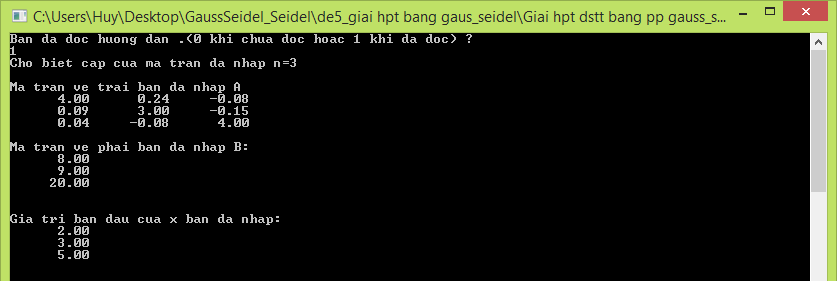
\includegraphics[scale=.7]{anh_3}
    \end{center}
    \caption{Hiển thị ma trận A, B và nghiệm xấp xỉ đầu $ X^{(0)}$}
    \label{refhinh1}
    \end{figure}
\end{center}

\begin{center}
    \begin{figure}[htp]
    \begin{center}
     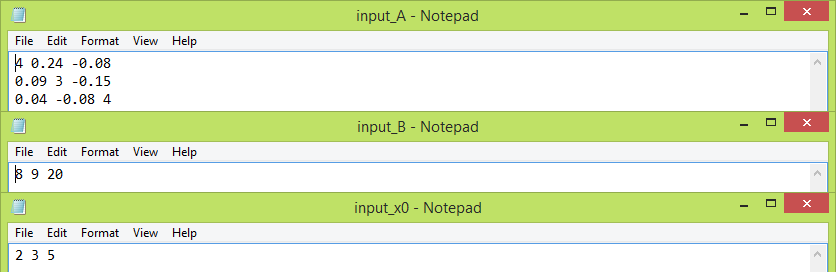
\includegraphics[scale=.525]{anh_6}
    \end{center}
    \caption{File "input\_A.txt", "input\_B.txt", "input\_x0.txt"}
    \label{refhinh1}
    \end{figure}
\end{center}

\newpage

\item Nhập sai số epsilon. Sai số nhập càng nhỏ thì kết quả trả về của các ẩn càng chính xác. Sau đó, màn hình console sẽ hiện ra tất cả các kết quả của từng vòng lặp tương ứng. Số vòng lặp nhiều hay ít phụ thuộc vòng sai số epsilon vừa nhập từ bàn phím. 
\begin{center}
    \begin{figure}[htp]
    \begin{center}
     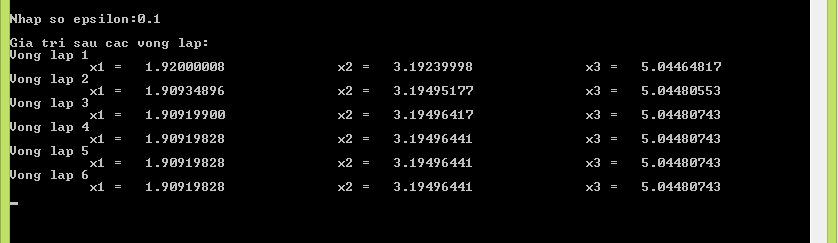
\includegraphics[scale=.7]{anh_4}
    \end{center}
    \caption{Nhập sai số epsilon và hiển thị kết quả}
    \label{refhinh1}
    \end{figure}
\end{center}

\item Kết quả cuối cùng sẽ được lưu vào file "output.txt".
\begin{center}
    \begin{figure}[htp]
    \begin{center}
     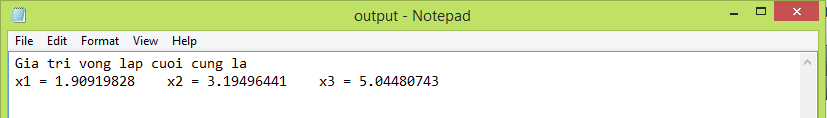
\includegraphics[scale=.7]{anh_5}
    \end{center}
    \caption{Lưu kết quả vào file "output.txt"}
    \label{refhinh1}
    \end{figure}
\end{center}

\end{itemize}
\end{itemize}

}
\newpage
\section{Nhóm báo cáo} 
{\renewcommand{\labelitemi}{$\blacksquare$}
\renewcommand\labelitemii{$\nabla$}
\renewcommand\labelitemiii{$\square$}

\hspace{0.7cm}- Nhóm báo cáo gồm 3 thành viên:\\

\\

\hspace{0.7cm}1. Phan Huy Hoàng ( nhóm trưởng ) - Tìm hiểu đề tài, viết báo cáo.\\

\\

\hspace{0.7cm}2. Trần Thị Thanh Tâm - Tìm hiểu đề tài, thuyết trình.\\

\\

\hspace{0.7cm}3. Nguyễn Văn Thành Dũng - Viết code chương trình.\\

\\

- Các công việc mà nhóm đã thực hiện khi tìm hiểu đề tài:\\

\begin{itemize}

\item{\textbf{Đọc - hiểu đề tài :}}
\begin{itemize}

\item - Nhóm đã dựa vào những kiến thức có sẵn trong giáo trình Giải tích số, kết hợp với đó là tìm hiểu thêm các thông tin ở trên mạng phục vụ cho bài thuyết trình và viết chương trình trên máy.\\

\item - Bên cạnh đó, thì trong 1 tuần tìm hiểu, nhóm cũng đã họp để thống nhất đề tài, bổ sung những phần lí thuyết còn thiếu, phân chia đầu việc chuẩn bị cho bài thuyết trình trên lớp.\\

\end{itemize}

\item{\textbf{Thuyết trình - Chạy code chương trình:}}
\begin{itemize}

\item Nhóm cũng đã chuẩn bị phần slide và code để trình chiếu, tuy còn chưa được hoàn chỉnh. Dưới sự góp ý của giáo viên bộ môn, nhóm cũng đã rút kinh nghiệm và chỉnh sửa lại trong phần báo cáo lần này.\\
\end{itemize}
\item{\textbf{Viết báo cáo:}} Trong báo cáo bao gồm những phần chính như sau: 
\begin{itemize}

\item Lý thuyết chung của phương pháp lặp Seidel và Gauss - Seidel.\\

\item Chạy chương trình trên máy.\\

\item Hoạt động của nhóm, phân chia đầu việc từng thành viên.\\

\item Tổng kết, ưu nhược điểm của phương pháp.\\

\item Code chương trình.\\

\end{itemize}
 

\end{itemize}
}
\newpage

\section{Kết luận}
{\renewcommand{\labelitemi}{$\blacksquare$}
\renewcommand\labelitemii{$\nabla$}
\renewcommand\labelitemiii{$\square$}

\begin{itemize}

\item Qua quá trình tìm hiểu đề tài, các thành viên trong nhóm cũng đã có kiến thức cơ bản về phương pháp lặp Seidel và Gauss-Seidel. 

\end{itemize}

\begin{itemize}

\item Ưu điểm: 
\begin{itemize}
\item Đối với phương pháp Gauss-Seidel hay còn được gọi là phương pháp lặp cải tiến có {\color{red}độ chính xác cao} và {\color{red}tốc độ hội tụ nhanh hơn} phương pháp lặp đơn (vì $\lambda < ||\alpha|| < 1$ )\\

\item Phương pháp Seidel {\color{red}tiết kiệm bộ nhớ hơn} phương pháp lặp đơn vì chỉ sử dụng n ô nhớ thay vì 2n ô nhớ cho $X^{(k + 1)}$ và $X^{(k)}$.\\

\item {\color{red}Dễ lập trình}. Chuẩn  $ || \alpha || $ càng gần 1 thì tốc độ hội tụ càng nhanh, nghiệm càng chính xác hơn.\\
\end{itemize}
\item Nhược điểm:
\begin{itemize}
\item Không phải tất cả các phương trình có nghiệm đều hội tụ nên việc sử dụng phương pháp lặp Seidel và Gauss - Seidel là không khả thi. Điều kiện đủ là chuẩn $ || \alpha || $ nằm trong khoảng $(0, 1)$\\

\item Nếu hệ số hội tụ quá bé ( $ || \alpha || << 1 $, gần 0 hơn ) thì ma trận sẽ lâu hội tụ về kết quả.\ Khi đó việc sử dụng phương pháp lặp đơn để giải hệ phương trình ĐSTT là tối ưu hơn.
\end{itemize}
\end{itemize}

}
\begin{center}
\bfseries 
{---HẾT---}
\end{center}
\newpage

\end{document}    %kết thúc tài liệu
